\chapter{Introduction}
\label{chap:introduction}

%{\em *** Version: \today~ ***}





%								
%								
%								



\bl
\o High-level introduction to thesis (Will be added when all chapters are more or less finished)
\el
% juice tiger?

\bc
Editing is concerned with the creation and maintenance of documents.  
Most documents have some form of structure. 
\ec
% Many applications are editing. view document, enter text, copy paste, move parts, navigate. 
% By abstracting over the specifics of the editor, a generic editor could offer a lot of advantages
% Only one editor for a range of documents provides a uniform interface, and makes embedding documents easy.
% moreover XML: lot of specialized documents that require editing. 
% Even though big ones are hard to replace, generic editor can create easily custom editors with advanced functionality
% Proxima is a generic editor with a number of features that make it possible to apply it to a wide range of applications

% Although the research in this thesis is not specifically tailored for XML, many of the results apply to XML as well, since 
% XML documents are tree structured documents. 


% identify problems, and propose an architecture with several novel features that .

% prototype has been implemented and although still lot of work to do. It already makes it possible to create editors
% in very little time

% maybe borrow from {Why Proxima} section
% also see ch_conclusions

*** The pictures in this chapter are still drafts because they might be replaced by screen-shots of the prototype.\\

\section{Preliminaries}

\subsection{Structured documents} \label{sect:structdocs}


%\section{Structured documents}
%Basics of XML and DTD's  Schema. CSS. XSL
%XML is EBNF 
%Documents are trees

A {\em structured document} is an amount of data that is composed of logical entities, between which a structural relation exists. Examples of structured documents are an HTML pages, program sources, word processor documents, etc. 

In this thesis, we restrict ourselves to structured documents that have a tree stucture that can be described by an EBNF grammar. Although graphs can be viewed as structured documents as well, algorithms for performing computations over graphs are far more complex than tree algorithms. Furthermore, parsers for graphs are less well understood than parsers for trees, as well as computationally much more expensive. 

We assume that the structure of a document is described by a formalism comparable to an EBNF grammar. In the cases where we explicitly want to describe the structure of a document fragment, we use simple Haskell~\cite{peytonJones03haskell} data types without higher-order types, except for the list type. Example document fragments are represented by Haskell terms. For example, a document representing the expression  $(1+2) \times (3 + 4)$ can be denoted in Haskell by: 

$Product~(Sum~(Int~1)~(Int~2))~(Sum~(Int 3)~(Int~4))$

\subsection{XML}


The eXtensible Markup Language XML~\cite{xml11} is an increasingly popular standard for representing structured documents. The standard is a simplified descendent of SGML~\cite{sgml86} (Standardized General Markup Language). XML documents are tree structured. The nodes of the tree are referred to as {\em elements}. The leaves of the tree are text or attributes (name-value pairs describing properties of an element). The tree structure is represented with opening and closing {\em tags}, and if these tags are nested correctly, the XML document is {\em well-formed}.

The expression example of the previous section may be represented in XML as:

\begin{scriptsize}
\verb|<Product><Sum><Int val=1><Int val=2></Sum><Sum><Int val=3><Int val=4></Sum></Product>|
\end{scriptsize}

The type of an XML document can be specified in several formalisms. The {\em Document Type Definition} (DTD) is part of the XML specification, and basically describes an EBNF grammar over XML elements. A much more expressive formalism is XML Schema~\cite{xmlSchema1}, which itself is a subset of XML. Compared to the DTD formalism, the advantages of a Schema include more control over textual content, as well as a form of inheritence. If an XML document conforms to a certain DTD or Schema, it is called {\em valid}. A third standard, which is not as common as DTDs or Schemas is the Relax NG standard~\cite{relaxNG01}. Relax NG is a combination of Relax~\cite{relax01} and TREX~\cite{trex01}, and is based on regular expressions. 


%XML is not a meta language.
%Although XML is often referred to as a meta-language, this is not a very accurate term. Indeed, the DTD part of an XML document may %define a language, However, In general, an XML document does not define a language, but is an element of a language. It is only the DTD %description that defines a language. Hence, it would be more appropriate to refer to XML as a super-language.

The number of standards for subsets of XML, also referred to as dialects, is rapidly growing. Besides the already mentioned XML Schema, we provide a few more examples.

The Mathematical Markup Language MathML~\cite{mathml20} is a standard for describing mathematical equations and expressions. %Expressions in MathML can be encoded based on  meaning, as well as on presentation. Hence, $1+2$ can be represented either as a sum %element that has two integer child elements, or as a sequence of three elements: two integers with a plus operator in the middle. 
Technical documentation can be represented with the DocBook~\cite{walsh02docbook} standard, which exists for XML as well as for SGML. The standard can also be used for papers and books. Finally, we mention the XHTML~\cite{xhtml11} standard, which is an XML encoding of HTML. Although similar, an HTML document is not necessarily an XML document, since HTML is a subset of SGML rather than XML.


%\note{mention how this thesis relates to XML?}
%** how this thesis applies to XML
%\fromHere

%\verb|<P>Some text with <b>bold</b> and <i>italic</i> words|
%$Para [Text "Some text with", Bold (Text )]$

%Difference between XML and Trees?
%%Difference XML is markup. CFG is tree, everything is part of tree. Markup is more document with tags. leads to differences. 
%things like expressions are awkward to model in XML. On the other hand, mixed... text with bold and bla tags are harder to describe in a %cfg, ...

\subsection{Editing}
\label{sect:editing}


%what is an editor
While the term {\em editor} is usually only associated with text editors such as Emacs~\cite{stallman81emacs}, we will use it in a much broader sense. We regard as an editor any application that shows an image of an internal data structure to a user and allows the user to modify this structure. The internal data structure is referred to as the {\em document} and the image is the {\em presentation}. 

%boundaries of editor concept
Naturally, word processors, image editors, and text editors are regarded as editors in this view, but there are also some less obvious examples. Take for example the preferences pane that is part of most window-based applications. The check boxes, selection lists, and text fields can be seen as a presentation of the preferences of the application. Another example of an application that is not usually regarded as an editor is a file browser.


\begin{figure}
\begin{small}
\begin{center}
\begin{center}
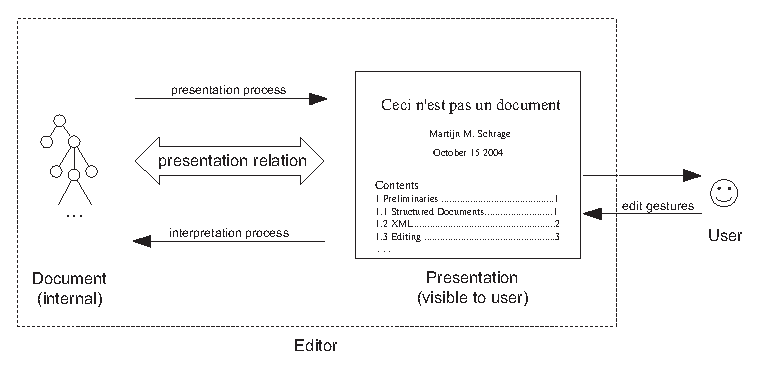
\epsfig{file=pics/eps/editor.eps, width=10cm}
\end{center}\caption{Schematic representation of an editor}\label{editor} 
\end{center}
\end{small}
\end{figure}

% document and presentation
Figure~\ref{editor} contains a schematic representation of an editor. The main data structures in the editor (also referred to as {\em levels}) are the internal {\em document} on the left and the user visible {\em presentation} on the right. The document is an internal data structure, which is not directly visible to the user. It should not be confused with a file, which is basically a presentation stored on a file system. Furthermore, we also do not consider an XML source to be a document, but rather textual presentation of the internal document.

\bc define levels \ec

A {\em presentation}, or {\em view} is the only thing a user sees of the document. A presentation may be textual, graphical, or a combination of both. We focus on static presentations only. Hence, we do not explicitly consider presentations containing sounds or animations, unless presented statically (e.g.\ as a textual link to a sound or video file). In the presentation, the editor shows the focus of attention, or {\em focus}, which is a shared name for the selection as well the cursor (which is an empty selection).  Several presentations of a single document may be shown simultaneously by the editor, each having its own focus. Finally, if a presentation resembles the final physical appearance of the document when it is printed, it is referred to as a WYSIWYG presentation (What You See Is What You Get).

% what is presenting
The relation between a document and its presentation is denoted by the term {\em presentation relation}, or {\em presentation mapping}. If, according to the presentation relation, the presentation is a presentation of the document, we say that the {\em presentation invariant} holds. Computing the presentation of a document is called the {\em presentation process}, whereas computing a document from a presentation is called the {\em interpretation process}. Together, the two processes implement the presentation relation and maintain the presentation invariant.

%***  define valid presentation!!
\bc
When the presentation level is a presentation of the document, we refer to it as valid. This should not be confused with valid for XML documents which means type correct.
also in defs
\ec

% what is sheet
The presentation relation for an editor may be (partially) specified in a style sheet, or {\em presentation sheet}. A presentation sheet describes how elements of the document type are presented, and is a parameter of the presentation process. By modifying the sheet, user may influence the appearence of the document without having to modify the editor itself. A presentation sheet can be regarded as a parameter to the interpretation process as well, since the interpretation depends on the presentation specified in the sheet. Examples of style sheet formalisms are the Cascading Style Sheets (CSS)~\cite{css2} for HTML as well as XML, and the Extensible Stylesheet Language (XSL)~\cite{xsl10} for XML.

%what is the edit process
Generally speaking, editing consists of repeated interactive cycles of presenting and interpreting. The editor shows a presentation of the document together with the current focus of attention to the user. The user then provides the editor with an {\em edit gesture}, such as a key press or a mouse movement, which is interpreted to an update on the document. The document is then re-presented and shown to the user. The process is repeated until the user quits the editor. Chapters~\ref{chap:informalSpec} and~\ref{chap:formalSpec} provide a more formal description of the edit process.

\head{Document-oriented vs. presentation-oriented editing}

% doc-oriented vs pres-oriented 
Because edit gestures may be targeted either at the document or the presentation, we distinguish two kinds of editing:  {\em document-oriented editing} or {\em structure editing}, versus {\em presentation-oriented editing}.

% also say document editing/presentation editing?

On the one hand, we have {\em document-oriented editing}, which consists of edit operations (including navigation and selection) that are targeted at the structure of the document rather than at its presentation. Examples are swapping two chapters in a word processor, selecting an entire chapter, or navigating to a next section.

On the other hand, {\em presentation-oriented} editing, consists of edit operations on the presentation, which do not necessarily make sense at the document level. If a presentation is textual,  presentation-oriented editing amounts to freely editing the text. As an example, take the mathematical expression from Section~\ref{sect:structdocs}: $(1+2) \times (3+4)$. Deleting the middle part $(1+\framebox{$\,2) \times ($}\,3+4)$, yields $(1+3+4)$, and is a presentation-oriented edit operation that is not a logical operation on the document level. Another example is navigating downwards in a formatted paragraph of a word processor, since the concept of lines in a paragraph only exists at the presentation level. 

Section~\ref{sect:intrProcess} provides a more thorough discussion of both document-oriented and presentation-oriented editing. Furthermore, the section discusses editing at several other levels, which are introduced at the beginning of Chapter~\ref{chap:proxArch}.
%doc editing is usually also pres editing

\head{Kinds of editors}

%what is structure editor
The term {\em structure editor} is used to make explicit that an editor has document-oriented editing functionality (also including navigation). We do not make a sharp distinction between text editing and structure editing. Instead, we regard all editing as structure editing, but with a varying level of structure. A text editor can be seen as a structure editor with a very simple structure model: a string or a list of strings. 

%what is generic?
An editor is a {\em generic editor} if it is not specifically built for a single document type but can be used to edit a whole class of document types. A generic editor may be {\em instantiated} to yield an editor for a specific document type. Genericity can be achieved with a single generic editor that edits documents of arbitrary types, but also with an editor generator. An {\em editor generator} is an environment that generates an editor application based on descriptions of the document type and its presentation. Although a generator is not as versatile as a single generic editor, we view both as generic editors. 

%structure editor is not nec. generic
For brevity, we will often adopt the common practice that the term structure editor implies genericity as well. Still, structure editors that are not generic are quite common. A few examples are: equation editors, bookmark editors in web browsers, and file browsers. On the other hand, a generic editor is always a structure editor since it knows about the type of the document.


%??maybe introduce XML Editor here? and forward ref?

%who is the user of a generic editor?
In the context of generic editing, the term {\em user} is ambiguous. A user can either be an editor designer, who instantiates the generic editor for a specific domain, or a user that is editing a document. Unless explicitly stated otherwise, we use the term for the document editing user.


\bc
When regarded as an editor, more sophisticated input fields that incorporate parsers, may be used. Furthermore, normal undo/redo functionality is possible, instead of the course grained OK/Cancel model, which only allows accepting or ignoring all changes at once.
\ec

\bc
% misschien niet zo'n interessante para
With such a broad view of editors, it is possible to regard every application, and even an entire operating system as an editor. In essence, all a computer user does is give edit gestures with the mouse and the keyboard in response to the presentation on the computer monitor. In reaction to the edit gestures, the internal state of the computer changes, giving rise to a new presentation. 

% en nog een
There is no fundamental problem with this view, but we do not adopt it because a definition that is too broad does not help in finding appropriate abstractions for a generic structure editor. Therefore, we do not explicitly consider all applications to be editors, but adopt the view that many applications contain editors.
\ec


Because it is difficult to give a precise definition of a generic structure editor and because such a definition might be to restrictive, we will we will use a number of typical use cases to clarify what we mean be a generic structure editor. Section~\ref{sect:usecases} presents these use cases.


%								
\subsection{Classes of structure editors}

Three classes of structure editors are distinguished in literature: {\em syntax-directed}, {\em syntax-recognizing}, and {\em hybrid editors}. Syntax-directed editors mainly support edit operations targeted at the document structure, whereas syntax-recognizing editors support edit operations on the presentation of the document. A hybrid editor combines syntax-directed with syntax-recognizing features, but the term is not used consistently in literature. To avoid confusion, we will refrain from using the term hybrid, except in a brief discussion below.

\head{Syntax-directed Editors} 
% mention that structure editing is often source editing.

The first structure editors that were developed are the {\em syntax-directed editors}~\cite{reps84synGen,Bahlke86PSG,magnusson90orm}, also known as {\em pure} structure editors. 

Early syntax-directed editors show a textual presentation of the document (usually a program source) but exclusively offer edit operations targeted at the internal document structure, and not at the textual presentation. The original idea behind this was that if structural edit operations were available, a user would not need the textual edit operations anymore. Worse still, presentation-oriented edit operations would interfere with the user's structural model of the document and introduce errors. Hence they were prohibited altogether. Most editors for XML (see also Section~\ref{sect:xmlEditors}), as well as editors for preferences panes can be regarded as syntax-directed editors.

\begin{figure}
\begin{small}
\begin{center}
\begin{center}
\begin{small}
\noindent \xymatrix{
   \dataa{$Document$} \ar[dd]    &     \\
                                              & User  \ar[lu] \ar@{.>}[ld] \\
 \dataa{$Presentation$}  &   \\
}
\end{small}
\end{center}\caption{A syntax-directed editor}\label{synDirEdit} 
\end{center}
\end{small}
\end{figure}


Figure~\ref{synDirEdit} shows a schematic representation of a syntax-directed editor. The editor works by computing a presentation of the internal document structure, which is shown to the user together with a current focus of attention. The user provides an intended edit operation (edit gesture) on the document structure, from which a document update is computed. After the document is updated, a new presentation is computed, which is shown to the user.

If the editor supports clicking in the presentation to set the focus, the editor also needs to keep track of the origin in the document for each position in the presentation.

In the figure, the line between the user and the presentation is dotted because syntax-directed editors do not support edit operations on the presentation very well. Because the presentation is derived from the document, an edit operation on the presentation first needs to be mapped onto an edit operation on the document, which is difficult if the edit operation is not a logical operation on the document level.

A major problem with syntax-directed editors is the restrictiveness of the edit model (e.g.~\cite{vanter94practical,rubinNeal87design}). New structures are easy to create, but not as easy to modify. If a user wishes to change a while statement to an if statement, simply typing over the keyword is often not supported. 

Many syntax-directed editors offer a form of presentation-oriented editing by providing a freely editable textual presentation of (part of) the document, and applying a parser to the edited text. Some publications~\cite{teitelbaum81progSynth, minor90editing} refer to such editors as hybrid, but as we willl explain below, we still regard these editors as syntax-directed editors. 

Unless the two forms of editing are completely integrated, the textual presentation forces a user to work in a different mode of editing, which is referred to as {\em mode switching}. Mode switching does not solve the problem of restrictiveness adequately. Often, a separate window showing a text-only presentation is opened and before the mode can be switched back, the edited text has to be valid. Furthermore, separate modes require a user to be constantly aware of the current mode of the editor. The resulting increased cognitive burden has been shown to be a source of errors~\cite{sellen90modes}.

% mention problems?
\head{Syntax-recognizing editors} 

At the other end of the spectrum are the {\em syntax-recognizing} structure editors~\cite{budinsky85sre, ballance92pan}. A syntax-recognizing editor keeps track of the textual presentation of the document. The user can freely edit the text, and the editor tries to recognize the document structure by means of a parser. Once the text has been (partially) recognized, structural information, navigation, and, in some editors, edit operations are available.

\begin{figure}
\begin{small}
\begin{center}
\begin{center}
\begin{small}
\noindent
\xymatrix{
   \dataa{$Document$}     &     \\
                                              & User  \ar[ld] \ar@{.>}[lu] \\
 \dataa{$Presentation$} \ar[uu] &   \\
}
\end{small}
\end{center}\caption{A syntax-recognizing editor}\label{synRecEdit} 
\end{center}
\end{small}
\end{figure}

Figure~\ref{synRecEdit} schematically shows a syntax-recognizing editor. The user's edit operations are targeted at the presentation, which can be edited freely. The document is derived by parsing the presentation; hence the reversed direction of the arrow, compared to Figure~\ref{synDirEdit}.

For each element in the document structure, the editor needs to keep track of what parts of the presentation it corresponds to, in order to show structural information in the presentation, as well as support structural navigation.  When a document structure has been recognized, the presentation may show additional information using font and color changes, context-sensitive menus, tooltips, etc.

Similar to the syntax-directed editor, the picture of the syntax-recognizing editor in Figure~\ref{synRecEdit} also contains a dotted arrow. In this case, because the document is derived from the presentation, structural edit operations on the document are difficult to support. A document-oriented edit operation has to be mapped onto an update on the presentation, in such a way that parsing the updated presentation returns the intended updated document. Presentation information that is not stored in the document tree, such as whitespace and comments, has to be related to the document tree in some way, in order to put in the right place after a structural edit operation.

The main problem with syntax-recognizing editors lies in their limited applicability. Because the presentation needs to contain enough information to derive the document, interesting presentations that only show part of the document are hard to support. Furthermore, graphical presentations, as well as presentations containing computed values and structures do not fit the model, as these are difficult to parse. As a result, syntax-recognizing editors are mainly limited to text-oriented applications, such as program source editors.

% mention: good for program editing?
\head{Hybrid editors} 

The term hybrid editor is used for an editor that supports structural edit operations as well as presentation-oriented (often just textual) edit operations.

In some publications (e.g.~\cite{teitelbaum81progSynth, minor90editing}), the term hybrid is used to refer to syntax-directed structure editors that have a limited form of syntax-recognizing functionality. As a consequence, most syntax-directed editors would qualify as hybrid editors, because most editors support some form of text parsing.

Others (e.g.~\cite{ballance92pan, koorn92gse}), however, advocate that the term hybrid should be reserved for editors that support full textual editing of the document, as well limited syntax-directed functionality, even if structural modifications on the document are not supported. In this view, almost all syntax-recognizing editors would classify as hybrid editors, since most of these editors support a form of structural navigation.

Because of this confusion, and because of the strictness of the syntax-directed versus syntax-recognizing classification, we refrain from using the term hybrid. Instead, we refer to editors that primarily support document-oriented edit operations as syntax-directed editors, and to editors that primarily support presentation-oriented editing as syntax-recognizing editors.

\subsection{Terminology}

We give a summary of the terms that were introduced in the previous sections.

\begin{description}
\item[Editor:] Application for creating and modifying documents. In this thesis also used to refer to {\em structure editors} and {\em generic editors} (or generic structure editors).
\item[Document:] Internal data structure that represents the information that is edited.
\item[Presentation/View:] Visible representation of the document.
\item[Presentation mapping/relation:] The relation between the document and its presentation.
\item[Presentation-oriented editing:] Edit operation targeted at the presentation: e.g.\ deleting $+$ from $1+2$, yielding $12$.
\item[Document-oriented editing/structure editing:] Edit operation targeted at the document: e.g.\ swapping two sections in an article.
\item[Presentation sheet:] Parameter to the presentation (and interpretation) process. 
\item[Presentation process:] Process of computing the presentation of a document.
\item[Interpretation process:] Process of computing a document from a presentation.
\item[Structure editor:] An editor that has knowledge of the structure of the edited document. Usually assumed to be a {\em generic editor} as well.
\item[Generic editor:] An structure editor that is suitable to edit documents of different types.
\item[Syntax-directed editor:] An editor that primarily supports document-oriented editing.
\item[Syntax-recognizing editor:] An editor that primarily supports presentation-oriented editing.
\end{description} 


%								
\subsection{Advantages of a generic structure editor}

An editor that knows about the structure of the edited document can offer interesting functionality. We list several advantages of generic structure editors. The first two advantages stem from the genericity of the editor, whereas the rest are mainly about the structural (document-oriented) abilities.

\begin{description}
\item[Uniform user interface/edit model.] Rather than a separate editor application for each type of document, a single generic editor can be used for a range of document types. Thus, instead of several slightly different interfaces, a user only needs to deal with a single uniform interface and edit model.

\item[Integration of documents.] Besides offering editors for different types of documents, a structure editor also facilitates the integration of different types of documents in a single editor instantiation. Thus, it is relatively easy to build an editor for a specific document type, with advanced functionality for the different kinds of edit. Examples are a word-processing editor with spread sheet functionality, or an editor for slide shows that has syntax coloring and type checking for program code appearing in the slides.

\item[Different Views on the Document.] A structure editor may provide a user with several editable views on the document. The views can show the document in a different order, or with a varying amount of detail. 

\item[Graphical Views.] A view may contain color and fonts in order to clarify document structure, but also use layout alignment, and graphical elements such as lines and boxes.

\item[Derived Information in the Presentation.] The editor can analyze the document during editing and display information computed from the document structure. Examples are the results of static analysis and type checking in source editors, but also chapter numbers or an automatically generated table of contents.

\item[Structural Edit Operations.] Some operations, such as demoting a section with subsections to a subsection with subsubsections in a scientific article, are straightforward to specify at the structural level, but awkward at the presentation level.

\item[Structural Navigation.] Navigating over the document structure instead of its presentation can be very useful. In a source editor, when the focus is on an identifier, a user may easily navigate to its definition in the source. Furthermore, an outline view of the document can be shown in which a user can click to navigate to the corresponding position in the document.

\item[Integration with Other Tools.] A structure editor allows fine control over integration with other tools, such as spell checkers, theorem provers, and program transformation systems. Furthermore, the editor may show the results coming from these tools at the appropriate position in the presentation, rather than as a list of messages with line numbers.


\end{description}

For document types with a textual presentation, such as program sources or XML documents, some of the advantages can be simulated with a text editor. Lexical analysis can be used on the edited text, and basic support for syntax coloring, auto-completion, and navigation can be provided. However, although simple and efficient, these solutions are  very basic and prone to errors, because, in general, much of the structure of a document cannot be recognized at a purely lexical level.

\bc
sometimes basic structural navigation.  Even though some of the document structure can be recognized at lexical level, in the general case, a full parse is needed. For example, when trying to specify a Haskell function definition as a line in which a '=' character is present, also lines containing strings or comments with '=' characters are identified as funcion definitions. In some cases the problems can be overcome, but in general this amounts to building a parser in a formalism that is too weak for that purpose. Therefore, we will not consider text editors in this overview of editors.
%*********************************
\ec

Despite the advantages, generic structure editors are not widespread at all. Several structure editors are used in small communities, but most development projects have been terminated, and in the last decade, very few publications on the subject have appeared. The rise of the XML standard has spawned a large number of generic editors, but when regarded as structure editors, XML editors do not show much variation and do not offer many of the possibilies that a structure editor could offer. Hence, their applicability is limited, and using an XML editor to edit a Java program source, for example, is not possible with the current generation of editors.

% maybe say we  explain why this is the case
% maybe say we will change it? or put that in outline?

% pan article


%\section{Why Proxima}
%
%(Will be added when all chapters are more or less finished)

%Why proxima
\bc
complex, but:
new stuff:

-extra state
-also editing on all? levels

Document standard XML getting popular, need editors.

interactive transformations, proof editors, rewrite systems
structural data complex presentations: math
programs with types and structural edit ops: IDEs

Proxima not about changing the world: struct editors, views.  editors have illogical/inconsistent features. Easiest to start all over with new model, however will frustrate users. Better to have a model that allow to express the familiar edit models. and merge them seamlessly.
\ec


\section{Outline of the thesis}

*** Will be added when all chapters are more or less finished ***

The outline of the remainder of this 

%As mentioned, users regard structure editors as being either overly restrictive, and/or not powerful enough.
Chapter~\ref{chap:requirements} explores the possible applications of generic structure editing, by providing five use cases of real-world editors. With these use cases in mind, we formulate a number of functional requirements that in our view are important for a flexible non-restrictive structure editor. The chapter also explains why current structure editors 
\bc
 I and then explore a number of functional requirements that in our view are important for creating a flexible non-restrictive structure editor.
\ec
\bl
\o Evaluation of editors
\o Introduction of Proxima
\el

The layered architecture of Proxima is introduced in Chapter~\ref{chap:proxArch}. The main data structures and components are discussed and examples of the presentation and interpretation processes are provided.
Chapter~\ref{chap:proxArch}:
\bl
\o Description of levels
\o Description of layers
\o Examples of presentation and interpretation
\el


Chapter~\ref{chap:informalSpec} 
Chapter~\ref{chap:formalSpec}

Chapter~\ref{chap:archCombs}
We discuss several methods of realizing connections between layers and abstract from one. Furthermore, explanation of layer in Proxima.

Chapter~\ref{chap:presenting} Important for editor.

Chapter~\ref{chap:prototype}

Chapter~\ref{chap:conclusions} presents the conclusions.  % Mention this one?
(Will be added when all chapters are more or less finished)
\bc
* mention here or in chapter proxArch?:
Bootstrapping problem, descr. of levels layers and edit model. second is easier to give with in a formal story. however, design reasons for first are hard to comprehend without idea. So first informal arch and edit model and later the formal stuff

\begin{itemize}
\item 2 Example editors, requirements and evaluation of editors according to requirements
\item 3 Explain the Proxima Editor
\item 4 Informal introduction to the specification
\item 5 Formal specification of a layered editor
\item 6 Haskell combinators for implementing the formal description
\item 7 The presentation formalism {\sc Xprez}
\item 8 The proxima prototype
\item 9 Conclusions
\end{itemize}



\ec